\chapter{Análisis literario -- II}
\label{sec:analisis-literario-ii}

\section{Potencias}

\lettrine[ante=\raisebox{-1.5ex}{\Large ---},lines=2]{M}{uy bien}
---arrancó Antonia---; nosotras queremos, entonces, generar ocho
esferas cuyos radios sean iguales a $\frac{\text{radio}}{2^i}$ y sus
alturas con respecto al origen sean iguales a
$\frac{\text{radio}\times 3\times (2^i-1)}{2^i}$, donde $i$ representa
la ubicación de cada esfera en la sucesión, contando desde 0. En otras
palabras, nos gustaría poder repetir algo como esto para cada valor de
$i$ entre 0 y 7:


    \begin{lstlisting}
translate([0,0,radio*3*(pow(2,i)-1)/pow(2,i)])
  sphere(r=radio/pow(2,i));
    \end{lstlisting}

    Cecilia se detuvo a considerar el texto. En primer lugar, Antonia
    reemplazó la altura (el tercer componente de la indicación
    \lstinline!translate!) por lo que parecía una expresión
    matemática: \lstinline!radio * 3 * (pow(2,i)-1)    / pow(2,i)!. Lo
    único desconocido por ella hasta el momento era la palabra
    \lstinline!pow!; supuso que tenía que ver con la potenciación.

 Antonia pareció leer su mente una vez más:
 
 ---Para expresar potencias en \openscad{} se emplea la función
 \lstinline!pow!\footnote{Quizá se deba a que en inglés potencia se
   dice \emph{power}. (Nota del Editor)}; la sintaxis genérica es
 \lstinline!pow(base,potencia)!. Por esa razón, \lstinline!pow(2,i)!
 es matemáticamente igual a $2^i$.

 \guillemotright Ahora bien ---recapituló Antonia---; deberíamos
 entonces repetir las dos líneas del texto anterior asignando a $i$
 los valores que van desde 0 hasta 7. En otras palabras, necesitamos
 crear una variable $i$ que tome \emph{todos} esos valores en
 sucesión, en lugar de uno solo.
 
 \section{Bucles}

 
 Antonia hizo un silencio pretendidamente teatral antes de continuar:
 
 ---Para lograr tan mágico y conveniente resultado nos valemos de la
 instrucción \lstinline!for!:


    \begin{lstlisting}
radio = 16;      

for (i = [0,1,2,3,4,5,6,7]) 
  translate([0,0,radio*3*(pow(2,i)-1)/pow(2,i)])
    sphere(r=radio/pow(2,i));
    \end{lstlisting}

    Cecilia casi no podía creerlo. <<¿Tan fácil era?>>, se
    preguntó. Según le pareció entender, la indicación \lstinline!for!
    asignaba a $i$, uno tras otro, los números encerrados entre
    corchetes, para con ellos crear las esferas correspondientes.

    ---Se puede mejorar un poco más ---Antonia interrumpió sus
    pen\-sa\-mien\-tos---. ¿No te parece molesto tener que escribir
    explícitamente cada uno de los números de la elemental sucesión
    aritmética que va de 0 a 7? No sólo es un poco molesto, sino que
    si quisieras hacerlo con 50 esferas, deberías
    escribir... demasiado, ¿no?

    Cecilia estaba tan contenta con lo conseguido hasta aquí que bien
    pudiera haber escrito la sucesión de 0 a 100 entera; pero entendió
    el punto de Antonia.

    ---Pues bien, eso se puede lograr; mirá ---prosiguió Antonia, cuya
    sonrisa crecía mientras escribía con Cecilia:


    \begin{lstlisting}
radio = 16;
      
for (i = [0:7]) 
  translate([0,0,radio*3*(pow(2,i)-1)/pow(2,i)])
    sphere(r=radio/pow(2,i));
    \end{lstlisting}

    \guillemotright Cinco líneas de texto, contando el espacio para
    separar visualmente las ideas ---la voz de Antonia no podía
    reflejar mejor la satisfacción que la embargaba, y Cecilia sintió
    que se contagiaba de la misma---; y si querés cambiar el tamaño de
    la base, o la cantidad de esferas, sólo debés modificar un valor:
    el 16 o el 7.

Antonia seguía leyendo el texto en silencio, como si buscara alguna
posible mejora, frunciendo los labios e inclinando la cabeza a uno y
otro lado. Finalmente dijo:

---Mirá, sólo para que lo tengas presente como posibilidad, te cuento:
quizás esas expresiones matemáticas un tanto extensas puedan
resultarte, cuando vuelvas al texto tras unos días, un tanto
oscuras. Podemos considerar la posibilidad de escribirlas usando
variables... a ver:


    \begin{lstlisting}
radio = 16;
      
for (i = [0:7]) {
  ri = radio/pow(2,i);
  zi = radio*3*(pow(2,i)-1)/pow(2,i);
  translate([0,0,zi])
    sphere(r=ri);
}
    \end{lstlisting}

    \guillemotright Recordá que la asignación de cada variable debe
    concluir con un punto y coma. Además, y debido a que ahora el
    bucle \lstinline!for! afecta a más de una instrucción (en este
    caso son tres: dos para las variables auxiliares y una para la
    creación del objeto trasladado) deben usarse llaves, a fin de
    encerrar con ellas el contenido que debe repetirse. Cuando el
    \lstinline!for! afecta a una sola instrucción pueden usarse
    también, pero no es necesario ---sentenció Antonia.

    Cecilia se moría de ganas de ver una torre de cincuenta
    esferas:


    \begin{lstlisting}
$fn = 200;
radio = 100;

for (i = [0:49]) {
  ri = radio/pow(2,i);
  zi = radio*3*(pow(2,i)-1)/pow(2,i);
  translate([0,0,zi])
    sphere(r=ri);
}
    \end{lstlisting}%$



\begin{figure}[ht]
      \centering
      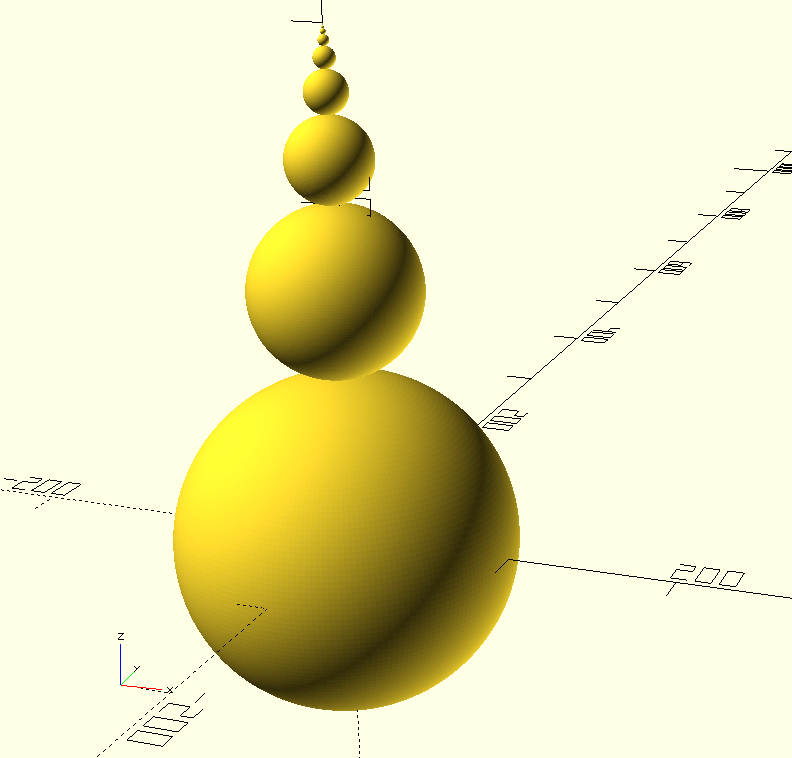
\includegraphics[width=.65\textwidth]{imagenes/50-esferas}      
      \caption{Cincuenta esferas apiladas por Cecilia usando un
        bucle. Lamentablemente, las progresiones geométricas se
        precipitan a valores ínfimos demasiado rápidamente, por lo que
        las últimas esferas no pueden apreciarse... ¡Aunque están ahí!
      }
      \label{fig:50-esferas}
    \end{figure}


    ---La última y terminamos por hoy ---prometió An\-to\-nia---;
    cuando declarás un bucle usando un rango, no es necesario pasar
    escrupulosamente por cada uno de sus valores; es posible indicar
    un `salto' entre uno y otro. De esta forma, si vos escribís
    \lstinline!for(i=[0:2:7])!, \texttt{i} toma los valores 0, 2, 4 y
    6; en otras palabras, vas avanzando de a 2:


    \begin{lstlisting}
$fn = 200;
radio = 16;

for (i = [0:2:7]) {
  ri = radio/pow(2,i);
  zi = radio*3*(pow(2,i)-1)/pow(2,i);
  translate([0,0,zi])
    sphere(r=ri);
}

\end{lstlisting} %$


\begin{figure}[ht]
  \centering
  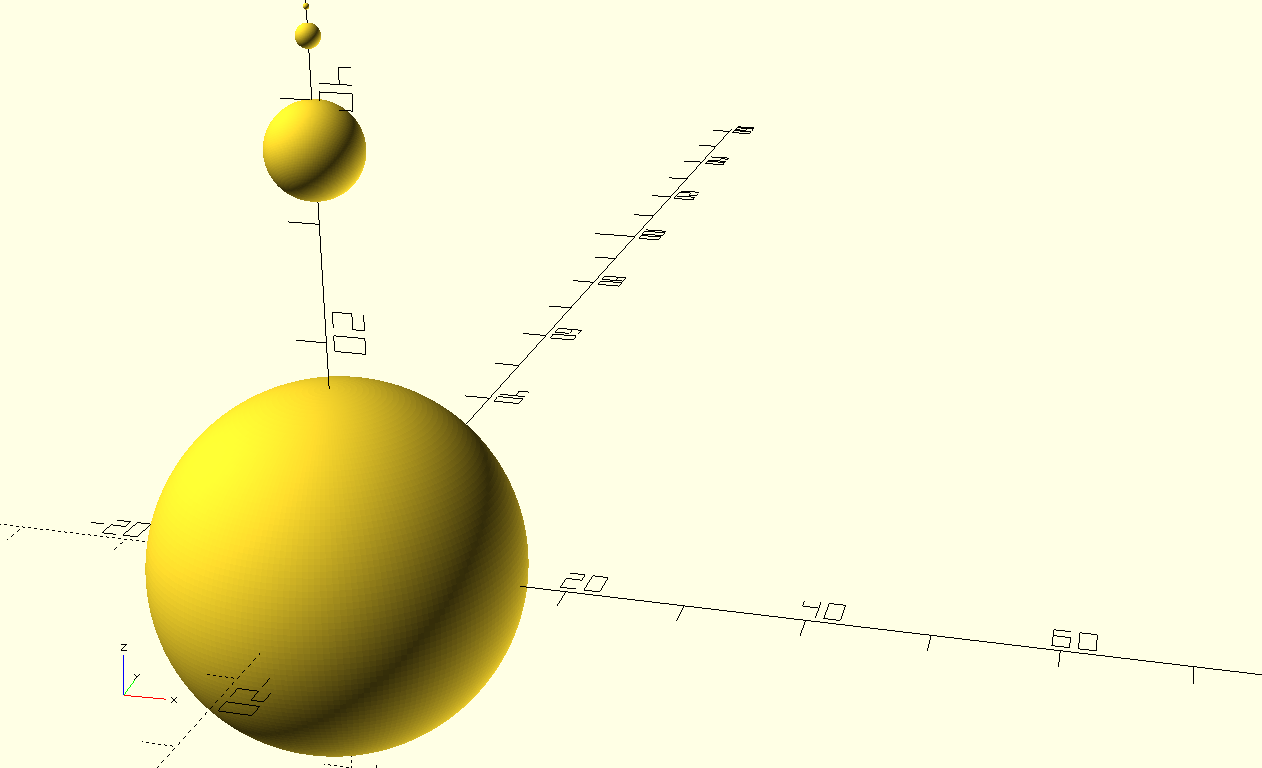
\includegraphics[width=.75\textwidth]{imagenes/esferas-alternadas}  
  \caption{Tres esferas alternadas.}
  \label{fig:esferas-alternadas}
\end{figure}

\guillemotright La sintáxis genérica es \lstinline!for(i=[inicio:paso:final])!. Por supuesto, el valor \texttt{final} puede
quedar excluido del rango si el \texttt{paso} es demasiado grande; tal
el caso que nos ocurrió a nosotras, donde el valor `7' resultó
omitido, ya que al `6' debería haber seguido el `8'.

\section{Desafío matemático}

Cecilia estaba feliz con la última versión del texto. Empezaba a
comprender porqué a Antonia le gustaba tanto programar. Ahora era ella
la que, casi sin proponérselo, leía y releía el texto en busca de
posibles mejoras. Súbitamente su atención recayó en los valores
numéricos empleados en las definciones de \texttt{ri} y \texttt{zi}:
esos `2' y `3' estaban claramente influidos por su voluntad inicial de
construir una torre donde cada esfera tuviera un radio exactamente
igual a la \emph{mitad} de la inmediata inferior... Eso tuvo como
efecto, además, que más allá de la octava o novena esfera las demás
resultaran imperceptibles. <<¿No sería genial que pudiera cambiar esos
valores para obtener una torre que respetara otra progresión
geométrica cualquiera?>> ---pensó---. <<¿Y que esos valores
dependieran de uno solo, que pudiera declararse al principio del texto
como una variable y en función del cual se calcularan los $ri$ y $zi$
correspondientes..? De esa forma, si el factor de decrecimiento fuera,
por ejemplo, 1,5, las esferas se parecerían más entre sí y la torre se
angostaría con mayor suavidad>>.

Cecilia confió a Antonia sus ideas, y ambas trataron de encontrar unas
fórmulas que las concretaran. Aún no lo consiguieron.\footnote{El autor
  de este librito confiesa encontrarse en la misma melancólica
  situación.}

\section{Una solución demasiado sofisticada}

Al día siguiente, Cecilia encontró a Antonia con gesto adusto y
distante. Preocupada, intentó indagar si algo malo le ocurría. Tras
mucho insistir, Antonia finalmente le confió su inquietud:

---Cecilia, logré que la torre crezca con un factor de
  decrecimiento cualquiera, a elección del usuario ---el tono
grave y serio de Antonia no condecía con lo que a Cecilia le parecía
una noticia excelente.

---¡Genial! ---Cecilia trató de sonar festiva, pero el gesto de su
amiga la cohibía un poco. Tras unos instantes, agregó
sua\-ve\-men\-te---: Antonia, ¿no deberías estar un poco más contenta?

---Pues... sí, es verdad ---Antonia, de mala gana, con\-sin\-\mbox{tió---.} El
problema es que usé una técnica un poco... sofisticada. No me siento
preparada para explicártela aún. Debemos compartir antes otros
recursos lingüísticos más elementales y básicos ---concluyó, con tono
de culpa.

Cecilia nunca dejaba de sorprenderse con Antonia: ¿eso la había
preocupado?

---¡Pero, che..! ¡Parece mentira! ---riendo, intentó
tran\-qui\-li\-zar\-la---.  Dale, al menos contame cómo lo pensaste
matemáticamente.

---Ah, bueno, eso sí ---Antonia recobró, de pronto, su
en\-tu\-sias\-mo---.  Como no fui capaz de hallar una fórmula de tipo
`cerrada', a la manera de la que conseguimos para el caso particular
de que las esferas decrecieran con un factor igual a 2, traté de
encontrar otra que reprodujera la expresión completa de la suma con la
que empezamos; ¿te acordás cómo venía? ---Antonia la escribió en el
pizarrón de su oficina:
\begin{align*}
  \text{Una esfera:}\qquad & zi = 0 \\
  \text{Dos esferas:}\qquad & zi = r+\frac{r}{k} \\
  \text{Tres esferas:}\qquad & zi = r+\frac{r}{k} + \frac{r}{k}+ \frac{r}{k^2}\\
  \text{Cuatro esferas:}\qquad & zi = r+\frac{r}{k} + \frac{r}{k}+ \frac{r}{k^2}+ \frac{r}{k^2}+ \frac{r}{k^3}
\end{align*}

\guillemotright En estas fórmulas `$r$' es el radio de la esfera
inicial y `$k$' el factor de decrecimiento, que en tu texto original
era igual a 2. Si te fijás, con cada nueva esfera se agregan dos
términos; dejame escribir una suerte de fórmula `general', en la que
uso paréntesis para destacar los términos que se agregan con cada
esfera:
\begin{equation}
  zi = r \cdot \left[ 0 + \left(  \frac{1}{k^0} + \frac{1}{k^1} \right) +
    \left( \frac{1}{k^1} + \frac{1}{k^2} \right) +
    \left( \frac{1}{k^2} + \frac{1}{k^3} \right) + \cdots \right]
  \label{eq:formula-torre}
\end{equation}

\guillemotright Pues bien ---y aquí el gesto de Antonia volvió a
en\-som\-bre\-cer\-se---, lo que hice a continuación fue escribir una
función que precisamente va sumando esos términos en \openscad{} para
cada valor de $i$.

---¡Guau! ¿Eso se puede hacer? ¡Excelente! ---Cecilia ensayó un
esfuerzo para conseguir que no decayera el entusiasmo de
An\-to\-nia---.  ¿Lo puedo ver?

Antonia se mostró inmediatamente muy esquiva; pareció querer
encerrarse en sí misma. Cecilia sabía que si eso pasaba, sería muy
difícil recuperarla:

---Dale ---rogó---; mostrame esa solución...

---Tengo miedo ---fue la lacónica respuesta que escapó de los labios
de Antonia, casi a regañadientes.

---Pero... ¿De qué? ---Cecilia preguntó, también con temor.

Antonia tardó en responder y, cuando lo hizo, con un hilo de voz, sus
ojos parecían querer escapar por la ventana de su oficina hacia los
jardines de Harvard:

---Pues... de que sientas que no entendés nada, te frustres, y salgas
corriendo de este libro.

Cecilia la miró unos instantes que parecieron una eternidad. Luego,
una sonrisa iluminó lentamente su rostro mientras decía, con un
marcado ceceo:

---Dale, zonza... moztrame eze texto de una
vez...

Antonia, desconcertada, pareció despertar bruscamente de un sueño,
hasta que la sonora risa de Cecilia la contagió.

---Bueno, está bien ---dijo Antonia, cuando sus risas finalmente se
apagaron---; pero conste que por ahora será sólo un texto que podrás
copiar y pegar sin entender, nada más. Te prometo, eso sí, que más
adelante y cuando hayamos visto otros temas más urgentes, vamos a
volver sobre él y desvelar juntas todo su significado. Sólo te
adelanto que en el texto, la variable \texttt{factor} se corresponde
con la `$k$' de las fórmulas anteriores ---Antonia se detuvo
dubitativa unos momentos, y agregó con un tono ligero---: ¡Quién sabe!
quizás incluso te resulte divertido jugar con los valores de la
variables involucradas, a ver qué onda.

    \begin{lstlisting}
$fn = 200;
radio = 16;
factor = 1.2;
for (i = [0:1:47]) {
  ri = radio/pow(factor,i);
  zi = z(i);
  translate([0,0,zi])
    sphere(ri);
}  
function z(i,acc=0) =
 (i==0) 
   ? radio*acc 
   : z(i-1,acc=acc+(factor+1)/pow(factor,i));
    \end{lstlisting}%$



    \begin{figure}[ht]
      \centering
      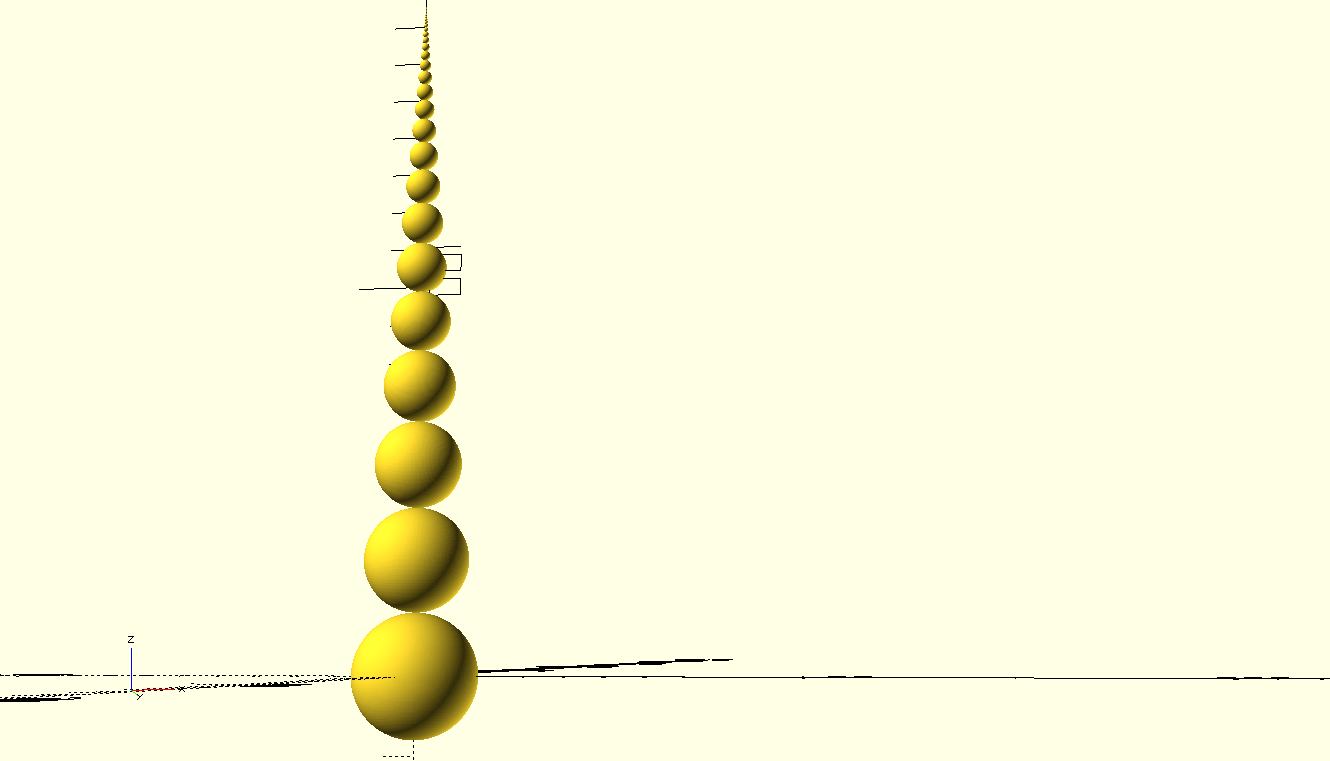
\includegraphics[width=.95\textwidth]{imagenes/muchas-esferas}      
      \caption{Una torre de muchas esferas.}\iftoggle{libro}{}{\vspace{128in}}
      \label{fig:muchas-esferas}
    \end{figure}

    A pesar de las advertencias de Antonia, Cecilia hizo un esfuerzo
    por comprender sola el texto anterior. No le sorprendió comprobar
    que no lo conseguía. Lo mejor que logró fue identificar
    oscuramente la expresión \lstinline!(factor+1)/pow( factor,i)! con
    esta otra: $\frac{k+1}{k^i}$, y ésta a su vez con el i-ésimo
    paréntesis de la fórmula \eqref{eq:formula-torre}:
    $\left( \frac{1}{k^{i-1}} + \frac{1}{k^{i}} \right)$. Sobre lo
    demás se cernía un velo opaco, demasiado pesado como para
    descorrerlo. Pero eso no la desanimó: antes bien, el suave
    contorno del párrafo escrito entre las líneas 10 y 13, aunque
    secreto y oscuro, lanzaba destellos como un desafío a sus ojos. Su
    corazón de científica volvió a encenderse ante lo desconocido, y
    la pulsión por entender la hizo vibrar una vez más.


%%% Local Variables:
%%% mode: latex
%%% TeX-master: "../libro"
%%% End:
